\documentclass{article}%
\usepackage[T1]{fontenc}%
\usepackage[utf8]{inputenc}%
\usepackage{lmodern}%
\usepackage{textcomp}%
\usepackage{lastpage}%
\usepackage[head=40pt,margin=0.5in,bottom=0.6in]{geometry}%
\usepackage{graphicx}%
%
\title{\textbf{Se registraron 983 protestas por derechos sociales en septiembre}}%
\author{El Nacional Web}%
\date{15/10/2018}%
%
\begin{document}%
\normalsize%
\maketitle%
\textbf{URL: }%
http://www.el{-}nacional.com/noticias/protestas/registraron{-}983{-}protestas{-}por{-}derechos{-}sociales{-}septiembre\_255843\newline%
%
\textbf{Periodico: }%
EN, %
ID: %
255843, %
Seccion: %
Protestas\newline%
%
\textbf{Palabras Claves: }%
Protestas, Sociedad\newline%
%
\textbf{Derecho: }%
2.1%
, Otros Derechos: %
2.2, 2.3, 2.10, 2.6, 2.8, 3.2%
, Sub Derechos: %
2.1.1, 2.2.1, 2.3.1, 2.10.1, 2.6.1, 2.8.1, 3.2.1%
\newline%
%
\textbf{EP: }%
SI\newline%
\newline%
%
\textbf{\textit{La organización indicó que 87\% de las manifestaciones fue debido a reclamos sociales~}}%
\newline%
\newline%
%
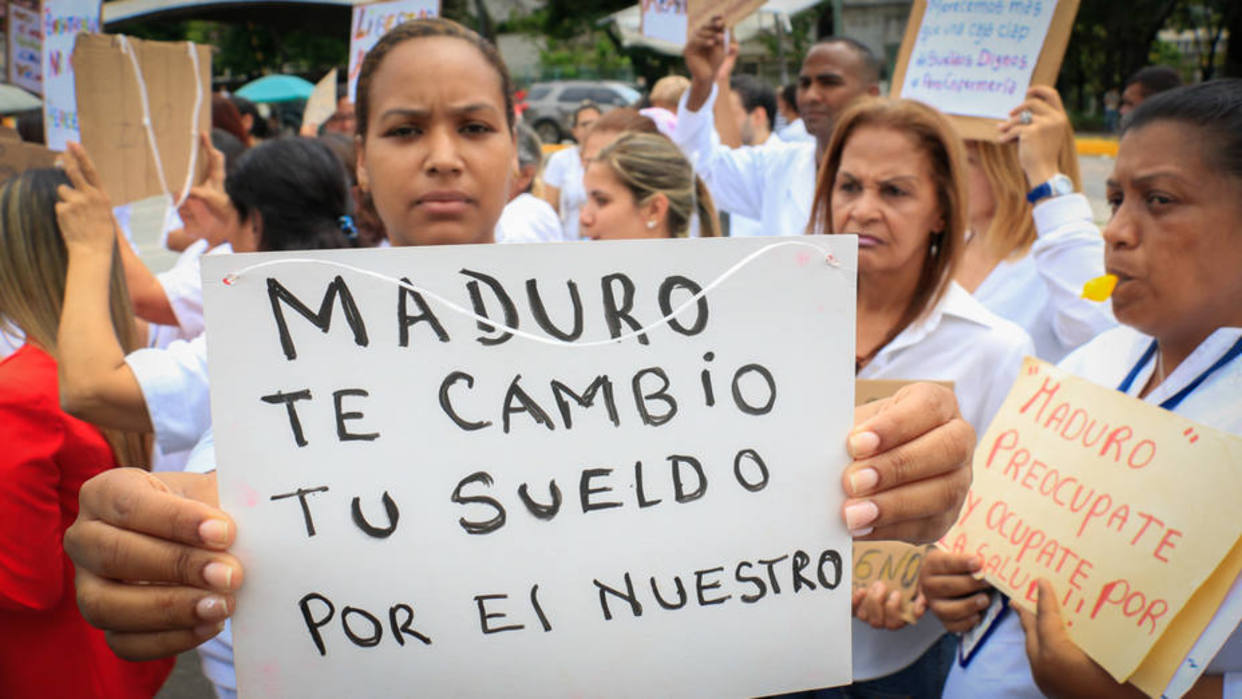
\includegraphics[width=300px]{150.jpg}%
\newline%
%
El Observatorio Venezolano de Conflictividad Social (OVCS) informó este domingo que durante septiembre se registraron 983 protestas en todo el país.~87\% de estas manifestaciones se deben a reclamos de derechos sociales.%
\newline%
%
La cifra publicada por el OVCS representa un incremento de 394\% respecto al mismo mes del año 2017, cuando fueron documentadas 199 protestas.%
\newline%
%
La organización indicó que las principales modalidades de protestas empleadas por la ciudadanía fueron el cierre de calles y concentraciones.%
\newline%
%
Los cinco estados en lo que se produjeron la mayor cantidad de protestas fueron: Bolívar, Táchira, Distrito Capital, Anzoátegui y Lara.%
\newline%
%
Para leer el informe completo ingrese~Aquí%
\newline%
%
\end{document}